%%%%%%%%%%%%%%%%%%%%%%%%%%%%%%%%%%%%%%%%%
% Master Thesis
% LaTeX Template
%
% Created by:
% Dániel Fehér
% If you have questions, feel free to contact me at:
% feher.dani46@gmail.com
%
% This is a LaTex template for the Master Diploma Thesis to use at the Eötvös Loránd University Faculty of Informatics, 
% EIT Digital Master School
%
% You are suggested to use it to write your EIT Digital Master Diploma Thesis at the Eötvös Loránd University
% Faculty of Informatics, EIT Digital Master School.
%
% You can modify this template, if you have improvements please send it to Zsófia Lovas (zslovas@inf.elte.hu)
%
% v1 28/04/2016 
%
% This work is licensed under a Creative Commons Attribution-NonCommercial-ShareAlike 4.0 International License.
%%%%%%%%%%%%%%%%%%%%%%%%%%%%%%%%%%%%%%%%%


\documentclass[a4paper,11pt]{report} % If you want to change the font size, you can do it here



\usepackage[utf8]{inputenc}
\usepackage[T1]{fontenc}
%\usepackage[latin2]{inputenc}
%\usepackage{t1enc}
\usepackage[english]{babel}
\usepackage{anysize}
\usepackage{amsmath}
\usepackage{amsfonts}
\usepackage{amssymb}
\usepackage{graphicx}
\usepackage{tikz}
\usepackage{algorithm}
\usepackage{algpseudocode}
\usepackage{epstopdf}
\usepackage{fancyhdr}
\usepackage{etoolbox}
%\usepackage {xcolor}  
\usepackage[table,xcdraw]{xcolor}
\usepackage{float} 
\usepackage{wrapfig}
\usepackage{url}
\usepackage{hyperref}
\usepackage{color}
\usepackage{tabularray}

\pagestyle{fancyplain}
\marginsize{3.5cm}{2.5cm}{2.5cm}{2.5cm}
\frenchspacing
\linespread{1.3} % If you want to change the line spacing, you can do it here

\fancyhf{}
\fancyhead[L]{\leftmark}
\fancyfoot[C]{\thepage}



\patchcmd{\chapter}{\thispagestyle{plain}}{\thispagestyle{fancy}}{}{}

\usepackage{ntheorem}
\theoremstyle{change}
\makeatletter
\theoremseparator{.}
\newtheoremstyle{theoremstyle}%
{\item[\hskip\labelsep\theorem@headerfont
            ##2.\ ##1\theorem@separator]}%
{\item[\hskip\labelsep\theorem@headerfont
            ##2.\ ##1\theorem@separator\ (##3)]}%
\theoremstyle{theoremstyle}
\newtheorem{theorem}{Theorem}[section]
\newtheorem{lemma}[theorem]{Lemma}
\newtheorem{claim}[theorem]{Claim}
\newtheorem{defi}[theorem]{Definiton}
{\theorembodyfont{\rmfamily}
\newtheorem{note}[theorem]{Note}
\newtheorem{conseq}[theorem]{Consequence}
\newtheorem{eg}[theorem]{Example}
}%
\newenvironment{proof}{\par\noindent{\bf Proof.}\enspace\ignorespaces}{~$\square$}
\makeatother



\def\myauthor{Bálint János Prágai} % Your Name
\def\mytitle{WIP:  Merkle Tree-based framework for verifiable and incentivized data contribution in
privacy-preserving recommendation systems: A Proof-of-concept} % Title of thesis
\def\myacdsup{Attila Papp} % Your Academic Supervisor from elte
\def\myacdsuptit{PhD Student}% Title of your Academic Supervisor from ELTE
\def\myacdsupen{Alexander Jung} % Your Academic Supervisor from your Entry University
\def\myacdsupentit{Title}% Title of your Academic Supervisor from your Entry University
\def\myentryuni{Aalto University}% Your Entry University
\def\myindsup{Johanna Viio Löfberg}% Your Industrial Supervisor
\def\myindsuptit{CEO}% Your Industrial Supervisor's title at its company
\def\myindcom{Fixmeapp AB}% Your Industrial Supervisor's company
\def\currentyear{2026.}% The Current Year

\definecolor{Gray}{rgb}{0.67,0.67,0.67}

\begin{document}

%%%%%%%%%%%%%%%%%%%
% Title Page - Don't Modify this! %%%%%
%%%%%%%%%%%%%%%%%%%

\begin{titlepage}
\pagenumbering{roman}
\thispagestyle{empty}

\textcolor{white}{}
\begin{wrapfigure}{l}{0.25\textwidth}
\vspace*{-30pt}
\includegraphics*[scale=0.25]{elte-logo.jpg}
%\vspace{-10pt}\vspace{-10pt}
\end{wrapfigure}
\vspace*{-30pt}
\begin{flushright}
{\fontsize{17.28}{20} 
\scshape Eötvös Loránd University\\}
{\fontsize{14}{10}
\scshape Faculty of Informatics}
\end{flushright}
\textcolor{white}{
\\
\\
\\
 \\
}
\vspace{2cm}
\begin{center}
{\fontsize{20.74}{20}  \scshape  \mytitle}
\end{center}

\vspace{4cm}

\begin{tabular}{p{9cm}c}

{\fontsize{14}{10} \scshape \myacdsup} & {\fontsize{14}{10} \scshape \myauthor}\\

{\fontsize{12}{20} \scshape  \myacdsuptit \ at ELTE}\quad & {\fontsize{12}{20} \scshape Data Science}\\

{\fontsize{14}{20} \scshape \myacdsupen}&\\

{\fontsize{12}{20} \scshape \myacdsupentit \ at \myentryuni}&\\

{\fontsize{14}{20} \scshape \myindsup}&\\

{\fontsize{12}{20} \scshape \myindsuptit \ at \myindcom}&\\
\end{tabular}

\vspace{3cm}
\begin{center}
{\large \scshape Budapest, \currentyear \\}
\end{center}
\end{titlepage}

%%%%%%%%%%%%%%%%%%%%%%%%%%%%%%
%%% Title Page ended, you can modify from here %%%%%%%
%%%%%%%%%%%%%%%%%%%%%%%%%%%%%%

\chapter*{Acknowledgement}
...

\tableofcontents

\chapter{Introduction}

\pagenumbering{arabic} %leave this here, to make the page numbering with arabic numbers from here

Current versions of data privacy oftentimes are opt-out models, giving users little control over their own data. The data is instead controlled by profit oriented organizations, profiling customers, exploiting them and their information, while the user receives no benefit from it. Usually combined with corner cuttings on safety (cite articles), this results in a bunch of Personal Identifiable Information (PII) (cite), that gives way to third party bad actors to reach an exploitable audience (cite), who should've been safe otherwise.\\
Furthermore, (cite) proved, that collecting all the information (via cookies or any other ways) is not even optimal and the surplus of data creates storage and analysis issues.
In this thesis I propose, that there exists an opt-in solution to replace primarily cookies. This Merkle-tree based, cryptographicaly secured system, that works in an ethical, human-centric way. (continue with structure)


\section{Relevance and problem definition}
[Same as in intro, but further detailed on ethicalties, examples from privacy policies, EU vs USA, cookies and web hooks/web beacons, inefficiency, data leaks and their dangers, avoidability]

\chapter{Literature review}
This thesis aims to create a framework for verifiable and incentivized data contribution system in privacy-preserving manner, to serve as a building block for an ethical data economy. 

After describing the methodology used for the reviewing of relevant past releases, this chapter introduces the relevant definitions and concepts starting with definitions in data marketplaces, data transactions and privacy.
The review follows with showcasing the findings from the keyword scanning of relevant terms.

\section{Review methodology}
To design a system, that can stand up to these standards properly, multiple search terms were examined for this literature review. First of the search terms is "ethical data economy". Exact keyphrase matching on Google scholar \cite{scholargoogle_ethicaldataeconomy2026} resulted in 26 papers found, that were published since 2016.
Using consensus.app \cite{consensus_ethicaldataeconomy2026} for extended keyphrase lookup, another 120 hits were found, making it altogether 146. After title relevance-screening, duplicate filtering and article access checks, only 39 articles remain. Abstract screening eliminated another 22, leaving us with 17.
The second search term is "merkle tree" AND "hash", where a similar technique, but only on consensus.app \cite{consensus_merkleandhash2026} resulted in ~5400 initial hits. After deduplication and keyword relevance filtering, the number of relevant articles decreased to 48, further decreasing to 10. Abstract filtering left us with 4 papers.
%TODO Flowcharts 


%consensus got 120 hits since 2016 (extended keyword search), google scholar found 26 since 2016 (exact keyword matching)
%google(19.03.2026.): https://scholar.google.com/scholar?q=%22ethical+data+economy%22&hl=hu&as_sdt=0%2C5&as_ylo=2016&as_yhi= 
%consensus.ai(19.03.2026.): https://consensus.app/search/ethical-data-economy/619aS1rJQoCezJx8dpjegQ/?utm_source=share&utm_medium=clipboard

\section{Ethical Data Economy}

Data became a 'hot commodity' as it keep gaining significance in our current world and is a basis for an economical system that dictates our lives. All the Machine Learning models are data hungry, making new models harder and harder to 'feed'. This resulted in some practices, that not all found human-centric, so call for ethical and human-centric data collection and handling practices grows ever louder.
One of the primary concerns laid out \cite{hyrynsalmi2023balancing} is the secondary data market, also known as data reselling. This is a problem concerning many data economy models and is the root cause of many transparency issues. Obviously it is a highly researched topic, but the consensus at the time of writing this thesis is that only software solutions can not protect against that.\\
%- Secondary data market usage \cite{hyrynsalmi2023balancing} <-> a system that hides the data itself, not the user\\

A couple of sources agree (\cite{valli2024ethical}, \cite{mirishli2025ethical}) that data economies are an ever-evolving landscape and should be treated accordingly. There should be constant exploration on what is happening, how data is used, how is it gathered and legal (e.g data and privacy protection laws) and ethical frameworks should constantly be recalibrated/reconceptualized. Similarly, current consent models are insufficient; consent for data gathering should be informed and adaptive. The research done by \cite{valli2024ethical} points to possible further explorations of data modification to achieve at least some of these goals. These are adding noise to the data artificially, consider different sensitivity for different kinds of data (e.g. treat phone number and health record protection differently) and exploring the privacy and utility trade-off, meaning the more private your data is, the less useful it is for systems. There should be some sort of balancing between the two, so all parties involved benefit the most.\\
%- prioritise transparent user mechanisms; use of federated learning; continuous recalibration and exploration; gaps: consideration of data sensitivity; privacy and utility enhancement trade-offs; adding noise to data \cite{valli2024ethical}\\
%- insufficient consent models; adaptive consent, regular reconceptualization of data protection laws \cite{mirishli2025ethical}\\

These demands for more ethicality in how our data is handled did not start that recently. Already back in 2018 there were demands formed on how data usage should benefit society. First, it should be clear who benefits from the data, all parties who do and, probably more importantly, who incurs the risk \cite{hand2018aspects}. This means knowing that in case of e.g a data leak, whose information is getting exposed and what kind of information (is it e-mails leaked or social security numbers or trade secrets?). The paper talks about how these thoughts motivated multiple organizations; The European Data Protection Supervisor (EDPS) places human dignity in the center, using it to balance out surveillance and asymmetry of power against the individual. The Data governance working group rather uses human flourishing as a 'guiding star'.  Meaning systems running on human created data, should be designed and governed in a way that it supports the well-being of humans (the ones creating the data). The author does warn, that ethics do differ region-to-region (for example different principles are considered ethical in UK than the EU  or the USA), so systems trying to conform to ethics should be aware of their 'audience'. The author also gives a checklist of what ethical data governance systems should consider. I don't give this list here, as later works define better considerations for the scope of the thesis.\\
%- be clear about who benefits who and who incurs the risk; EDPS: human dignity; Data Governance Working Group: human flourishing; ethics are not universal (EU vs UK vs USA); harm: health detriment, financial loss, discrimination, (gives and ethical checklist) \cite{hand2018aspects}\\
Rantanen and Koskinen started publishing in similar topics to the previous in 2019. Koskinen identified a gap in humanistic approaches to data governance, as demand started rising for it, especially in the EU \cite{koskinen2019if}. They identified the need for commonly accepted ground rules, which would start with a fair governance system (preferably an international one), sadly that is out of the scope of this thesis. Rantanen took a more down-to-earth approach, as they surveyed people's demand and expectation from an ethical data economy \cite{rantanen2019towards}. They found that people expect a system like this to support their autonomy, protect their privacy, to be secure and transparent, trustworthy, benevolent and just. As a whole they want it to be beneficial both to them as individuals and the rest of society.
%- people find these important: support autonomy, protect privacy, security, transparency, trustworthy, benevolent and just; beneficial to both individuals and society \cite{rantanen2019towards}\\
%- rising demand for more humanistic approaches; already some steps, at least in Europe; need for commonly accepted ground rules; starting point is fair governance, out of scope for this thesis \cite{koskinen2019if}\\
A year later, when talking about and defining a human-centric data economy, Rantanen et al. split human values into 2 groups: intrinsic and instrumental \cite{rantanen2020ethical}. Autonomy, justice and security of data are intrinsic values, while they categorized transparency, honesty and supervision instrumental ones. While their results are not absolute, they argue that these values should be included in a data economy that includes and is sustained by humans. Things that humans value should be studied more (and so should ways on how this can be done) for these claims to gain more rigor, but this paper defined a direction for a part of the studies on data economy ethicality up until now. 
%- autonomy, justice and security are intrinsic values to a data economy; transparency, honesty and supervision are instrumental ones; these values must be included in the human-centric data economy; gaps: how to study these, more and deeper studies on what we, humans value \cite{rantanen2020ethical}\\
In the same year they continued this study in \cite{rantanen2020humans} which was a study done on over 8000 people, 4792 of which gave really valuable answers, the summary of which can be found in Table \ref{tab:european_demand_summary}. There are 2 key takeaways here; The most pressing (and important) demand seems to be transparency, as not only large percentage of the participants demanded it, but is also enables the fulfillment of other demands, such as true control over data, informedness, security, trust or being in general aware of benefits. The second takeaway is that participants wanted an active role in a data economy; They want to have control over their data, be aware of what is happening to it (who can see it, who buys/uses it), benefit from the usage of their data and even in some cases the ability to supervise this system. The authors correctly identified a gap in communication between stakeholders at the time leading to large part of the demands. 
%- n = 4792 participants (non-representative of subgroups); \ref{tab:european_demand_summary}; 2 key takeaways: transparency is a demand and an enabler for other demands (true control, informedness, security, trust, be aware of benefits); active role: control over own data, be aware of what is happening to said data, benefit from this, maybe supervision of the systems; big pitfall is communication \cite{rantanen2020humans}\\
In their last paper of the year \cite{rantanen2020respecting} they built on the previous researchs' identified values and concluded, that human empowerment comes through information control. This means people should be able to control information about them; both what is visible and how it can be traded. To enable this, the paper suggests a good first step to be extending governance bodies to build trust in the whole data economy (stakeholder network).\\  
%- builds on prev paper on values; empowerment through information control; extend governance bodies to build trust in the entire network \cite{rantanen2020respecting}\\
The conclusion to their research saga would be their paper in 2023 \cite{koskinen2023ethical}. Here they discuss, how the current data economy practices and models are not in line with values of individuals and how there is a rising demand (and need) for an approach that follows ethical guidelines. They identified GDPR and similar frameworks have taken good steps towards this, but this is not enough. A good data ecosystem requires constant communication between stakeholders (as seen in \cite{rantanen2020humans}) and also facilitates it. This communication should focus on the data (and strategies) shared between these stakeholders. This constant communication would also enable regular restructuring of the system with active actors, as have been identified as a need previously. Their main point can be summarized in their quote: "Individuals are bypassed in the current data economy, which is strongly based on collecting from them." To achieve this, they identified a couple of next steps: The analysis and rethinking of current communication practices between stakeholders of data economies, research new, proper ways of effective communication and how viability of all this.\\
%- current data economy is not in line with values of individuals, a need for more ethicality has risen; GDPR and alikes has been taken as good steps, but not enough; a good ecosystem requires and facilitates constant stakeholder interaction (see: pages 8 figure of the article); focus on the data and strategies shared between ecosystem stakeholders; constant communication and potential restructuring with active actors; "individuals are bypassed in the current data economy, which is strongly based on collecting from them"; gap: current communication practices between stakeholders, proper way of this communication, viability \cite{koskinen2023ethical}\\

A different approach in values to Rantanen and Koskinen also emerged in 2019. Devitt et al. collected all together 15 goals/principles around 4 topics: community, rights, usability and politics \cite{devitt2019principles}. Community refers to the data subjects, who produce the personal data fueling the data economies; these economies should be for these subjects and preferably ran by them, including communal sharing of information and self-governance. Rights talks about data collection should respect human rights, benefit humans and the natural world. Usability is about the processing of the data and what it needs to be processable; it should be fit for purpose and useable, collected in a consensual, fair and transparent manner. Data is dependent on context (this context should be accounted for) and with reasonable exceptions it should be available to the public, to be revisable and form a useful social capital. Politics show how data can empower democratic people; data empowered people should be able to challenge existing political and economic norms, so they can revise this and achieve better, more equal and secure democracy. This approach was not as deeply researched as the one shown in the previous works, it does, however, consider the usability and transparency of the data and the seeming contradiction between them.\\
%- 15 principles: community: orchestrated and mediated by and for data subjects, including communal sharing for community decision making and self-governance; rights: should be collected with respect to humans and their rights and the natural world; usability: usable and fit for purpose; consensual, fair and transparent and must respect interpersonal relationships, data is dependent on context and with reasonable exceptions should be open and published, revisable and form useful social capital; politics: reveals and challenges the existing political and economic order so that data empowered people can secure good democracy. \cite{devitt2019principles}\\

The work of these authors made others evaluate the situation and come up with models for ethical data economies, especially in the age of AI and exponentially growing data demands. 
Hajoary et al. addresses identifies the gap between ethicality and data monetization combined with AI data consumption \cite{hajoary2023exploring}. They reviewed the concerning literature and found that while AI, data base, Machine Learning were popular (high number of published papers), Ethics, law, rights were less researched. In these they identified a human need of transparency for data collected from them. Finally they further reinforce the need for culturally and ethically sensitive data governance policies, mostly in the EU and USA.\\
%- data monetization and AI data consumption don't align with ethical theories, that concern them; theoretical, ethical and methodological advancements; keywords of ethic, law, right, database, ai were popular in publishing; transparency is a big takeaway in human needs; reinforced needs for culturally sensitive data governance policies (in EU and USA)\cite{hajoary2023exploring}\\

Moran approached the question from the Big Data side \cite{moran2022towards}; They identified a gap between tools available and Big Data. Currently the latter outclasses the former in most aspects, leading to a non-transparent, overly powerful tool. This means Big Data requires deeper contemplation and rethinking, possibly reimplementation. Big Data needs to be handled in a way, that it is in accordance with human autonomy, while avoiding the pitfall of overregulation and regulatory loopholes. The invasiveness and number of people affected suggests using group ethics as ethical framework for resolving some moral dilemmas regarding the topic. The article finally warns, that Big Data systems should be aware of these limitations and especially dilemmas when being designed and should hold up to ethical frameworks.\\
%- operational challenges: people to be trained on data; Big Data exceeds current tools in capabilities; services created on the search of information; Big Data requires deep contemplation; moral responsibility - implementation with accordance to human autonomy; fear/pitfall of regulatory loopholes and overregulation; resolving moral dilemmas; must be aware of these limitations, especially the dilemmas; invasiveness and number of people affected call for uses of group ethics\cite{moran2022towards}\\

Okorie et al. further reinforce the need for consent, transparency and privacy in ethical data economies \cite{okorie2024ethical}. Furthermore, they identified a need for adaptable and inclusive ethical frameworks. They reason these are addressing the complexities in the data subjects generating and affected by the data. They conclude that integrating ethical considerations into every step along the way of creating data economies is necessary, also can be referred to as 'ethical by design'.\\
%- consent and privacy are foundational elements for this; need for adaptable and inclusive ethical frameworks to address complexities; transparency; integrating ethical considerations into each and every step is necessary \cite{okorie2024ethical}\\

Keymolen and Taylor suggest putting responsibility on regulators and data scientists alike \cite{keymolen2023data}. They call for new regulations not only for data handling, but for those who are handling it. They argue data scientists should be accountable (as on go through rigorous evaluations, no political) as their work directly and indirectly influences the lives of large portion of the population. They reason, because of the magnitude of this impact data science and data driven businesses have on society, more ethical research and business practices should be enforced. (Significant impact on society includes education, social relations, news, buying habits, media.) Data ethics as is, is unfit for this, as complexity of data demands it having open definitions and somewhat lose rules. This allows for malevolence in the form of ethics washing, which is dangerous while the ethics washed systems can impact society in this serious of a manner. This means data ethics need a revisit and ethics washing should be avoided at all cost.\\
%- call for new regulations; responsible data scientists, accountable (rigorous evaluations), no political incentives; reinforcement on more ethical business practice and data handling demands; data science and data-driven business have ethically significant impact in society (education, social relations, news, propaganda, buying); data ethics has a lot of open and sucks at defining what is the right thing to do -> ethics washing is a real danger, should be avoided at all costs.\cite{keymolen2023data}

Somewhat connected, a study in 2024 proposed a framework integrating some previously mentioned results and demands \cite{von2024data}. The article proposes a definition of data sovereignty as "The capability of a natural person or legal entity for exclusive self-determination with regard to its economic data goods" and lists several aspects of it. They argue the essentialism of data sovereignty for trusted data sharing between individuals and organizations/legal entities. They conclude that this trust between the different parties is essential in order to enable effective innovation. \\
%- data sovereignty: The capability of a natural person or legal entity for exclusive self-determination with regard to its economic data goods (has 7 aspects and their relations); essential to guaranteeing trusted data sharing between individuals and organization of different parties to make innovation happen \cite{von2024data}\\

I, however, would argue that the next paper offers a better solution. Sohail et al. identify issues relating to individuals' matters \cite{sohail2024data}. These being data protection, fairness, transparency,  confidentiality, integrity and autonomy. There was a framework that was close to solving those at the time, FAIR (findable, accessible, interoperable, reusable). While it was adopted in some areas, for mass adaption FAIR or FAIR principles would require coordinated efforts from multiple stakeholders, involving governing forces like federal governments or even the EU. They suggest and improvement on the framework in the form of the FACT (fairness (not as previous), accuracy, confidentiality, transparency) principles. This was developed (and to some extent adopted) in the Netherlands. Their improvement to this framework is the use of something called an Open Personal Data Store (OpenPDS). This Open version of PDS over the regular is required, so that it aligns with company interest of not making all data public. (Important to note, that the study also shows enterprises holding onto data for longer doesn't make service any better. transparent and trustworthy companies are more likely to get data.) PDS allows for both queries and answers to happen in an encoded way, hiding data. OpenPDS further demands users have increased control over when they share data (privacy preservation and choice control) and this is how this system is the best we have so far.
%- issues relate to individuals' data protection, fairness, transparency, confidentiality, integrity and autonomy; solution (best, so far): FAIR(findable, accessible, interoperable, reusable) acclaimed and adopted; to achieve FAIR data, coordinated efforts from multiple stakeholders is required; FACT(fairness (not as prev), accuracy, confidentiality, transparency) developed and somewhat used in the Netherlands; Enterprises holding onto data for longer doesn't make service any better. transparent and trustworthy companies are more likely to get data; FAIR and OpenPDS(personal data store) --  data availability is not company interest; PDS is queried in code and answers in code; OpenPDS demands users have increased control over when they share data (privacy preservation and choice control) \cite{sohail2024data}\\




\begin{table}[H]
\centering
\caption{Summary of the demands surveyed by Rantanen and Koskinen (cited from \cite{rantanen2020humans})}
\refstepcounter{table}
\label{tab:european_demand_summary}
\begin{tblr}{
  row{1} = {t},
  row{2} = {t},
  row{3} = {t},
  row{4} = {t},
  hlines = {Gray},
  vline{2} = {-}{Gray},
  hline{2} = {-}{0.08em},
}
Theme                              & Demands for a fair data economy                                                                                                                                                                                                                                                                                                                                                                                                              \\
Control over data and data sharing & {\labelitemi\hspace{\dimexpr\labelsep+0.5\tabcolsep}Power over data sharing and content\\\labelitemi\hspace{\dimexpr\labelsep+0.5\tabcolsep}Preserving privacy\\\labelitemi\hspace{\dimexpr\labelsep+0.5\tabcolsep}Informed and dynamic consent\\\labelitemi\hspace{\dimexpr\labelsep+0.5\tabcolsep}Possibility to control the content (requires access)\\\labelitemi\hspace{\dimexpr\labelsep+0.5\tabcolsep}Easy-to-use control mechanisms} \\
Transparency and being informed    & {\labelitemi\hspace{\dimexpr\labelsep+0.5\tabcolsep}Transparency of processes\\\labelitemi\hspace{\dimexpr\labelsep+0.5\tabcolsep}Ability to see what is collected\\\labelitemi\hspace{\dimexpr\labelsep+0.5\tabcolsep}Comprehensible and on-going communication}                                                                                                                                                                            \\
Security                           & {\labelitemi\hspace{\dimexpr\labelsep+0.5\tabcolsep}Secure services\\\labelitemi\hspace{\dimexpr\labelsep+0.5\tabcolsep}Confidentiality, anonymity\\\labelitemi\hspace{\dimexpr\labelsep+0.5\tabcolsep}Transparent data management\\\labelitemi\hspace{\dimexpr\labelsep+0.5\tabcolsep}Better understanding of security}                                                                                                                     \\
Trust and fairness                 & {\labelitemi\hspace{\dimexpr\labelsep+0.5\tabcolsep}Trustworthiness of service providers\\\labelitemi\hspace{\dimexpr\labelsep+0.5\tabcolsep}Clear promises that are kept\\\labelitemi\hspace{\dimexpr\labelsep+0.5\tabcolsep}Fair treatment of all parties}                                                                                                                                                                                 \\
Compensation and benefits          & {\labelitemi\hspace{\dimexpr\labelsep+0.5\tabcolsep}Concrete benefits for disclosing data\\\labelitemi\hspace{\dimexpr\labelsep+0.5\tabcolsep}Common good\\\labelitemi\hspace{\dimexpr\labelsep+0.5\tabcolsep}Clear and honest communication about the~benefits}                                                                                                                                                                             \\
Supervision and rules              & {\labelitemi\hspace{\dimexpr\labelsep+0.5\tabcolsep}Rules and laws are obeyed\\\labelitemi\hspace{\dimexpr\labelsep+0.5\tabcolsep}Supervision of the system by an independent institution\\\labelitemi\hspace{\dimexpr\labelsep+0.5\tabcolsep}Sanctions if rules are broken}                                                                                                                                                                 \\
Negative attitudes                 & {\labelitemi\hspace{\dimexpr\labelsep+0.5\tabcolsep}Trust needs to be gained back\\\labelitemi\hspace{\dimexpr\labelsep+0.5\tabcolsep}More holistic approach than a label needed}                                                                                                                                                                                                                                                            
\end{tblr}
\end{table}

\section{Data marketplaces}
Data is a relatively new commodity \cite{haav2014data}. This means, that data markets and marketplaces were emerging in the 2010s, but as data was an unconventional product, the terminology across data sales was not uniform. \cite{stahl2016classification} successfully identified this gap and created a terminology framework that follows traditional market definitions, while adapting to this computer science environment. The following terminological framework will be used throughout this thesis;
\begin{defi}
    Market is an economic structure, the abstract place of trade, that serves three functions: Institute, transaction and pricing mechanism. As an institution market is a framework of rules, that assigns roles to its actors, as well as expected behaviors and protocols. The market is made up from the transactions happening in it, so the market defines these transactions. They consist of four phases; (1) Information phase (actors get informed about exchange intentions (bids/offers)), (2) negotiation phase (actors negotiate the product, contract terms and price), (3) transaction phase (contracts are fulfilled), (4) after-sales phase (customer service) \cite{richter2002elektronische}. As pricing mechanism, the market leads the actions of buyers and sellers and signal the conditions of sale to other participants. These definitions apply to electronic markets and in them to data markets. These only deviate in implementation of the institutionality and pricing philosophy as transaction costs are low and they are highly accessible.
\end{defi}
\begin{defi}
    An electronic marketplace the concrete virtual institution and place of exchange that brings together supply and demand and supports the trade between providers and customers, i.e., transferring the market function into an electronic infrastructure. Any type of business action on online platforms or any type of electronic venture falls into this dimension with no regard to whether they are based on competition or on collaboration.
\end{defi}
A data market and marketplace conform to the definitions above. Based on those \cite{stahl2016classification} define them in the following way:
\begin{defi}
    Data marketplace is an electronic marketplace, where:
    \begin{itemize}
        \item A provider's primary business model needs to be providing data and/or related services. 
        \item Data marketplace provider's need to offer an infrastructure that allows customers to upload, browse, download, buy, and sell machine-readable data. (e.g. CSV, XML, JSON) The data have to be hosted by the providers and it needs to be clear whether the specific data come from the community or the operator.
    \end{itemize}
\end{defi}

Furthermore, Figure \ref{fig:data_market_hier} shows the hierarchical analysis of the model proposed in \cite{stahl2016classification}, out of which this system could be either categorized as buy-side system or a buy-side platform, as the product (data) supply is in the hands of the platform owner. Many users individually produce data, but the platform owner collects it and offers it to the numerous, outside buyers. This warrants buy-side system as a better description of marketplace of the two. %TODO meeting with Johanna

\begin{figure}[H]
    \centering
    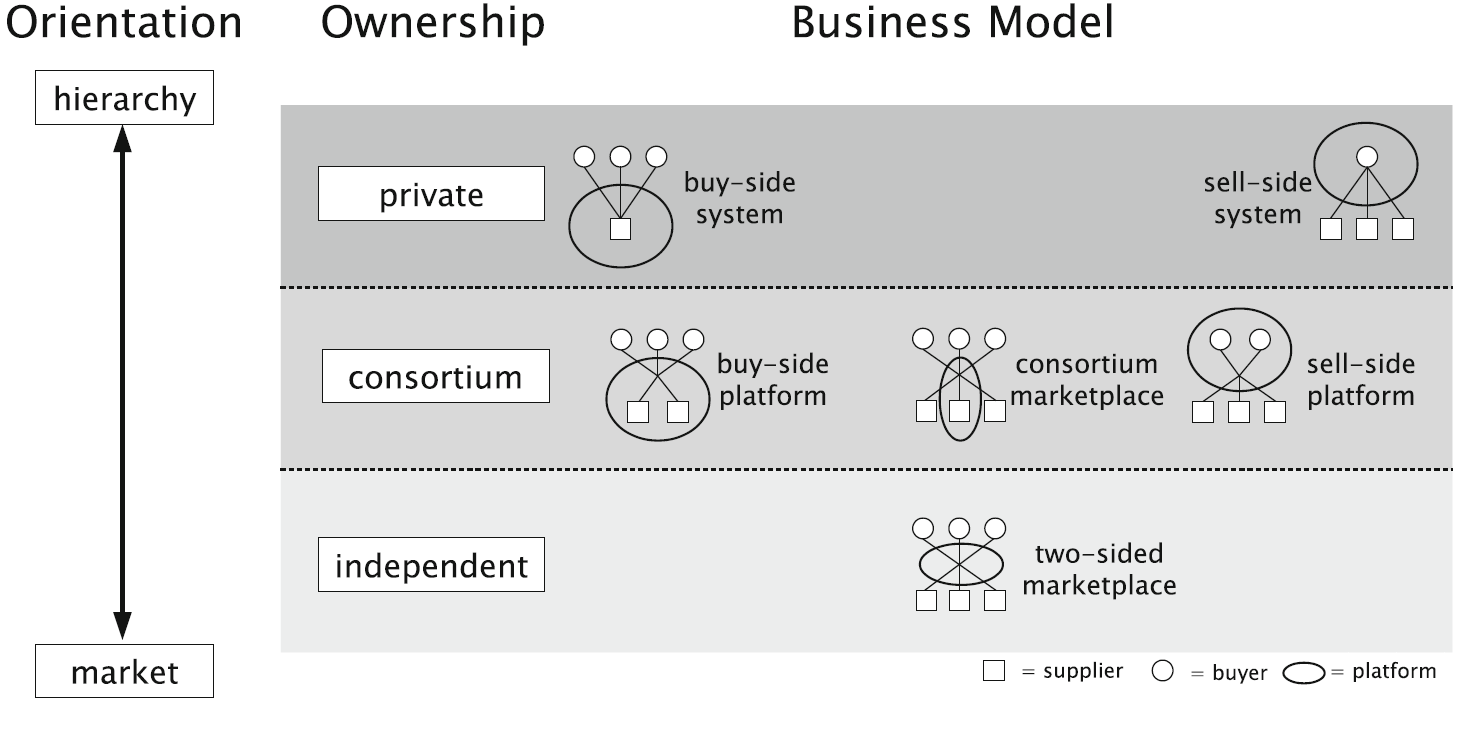
\includegraphics[width=1\linewidth]{datamarketdef.png}
    \caption{A model of electronic marketplaces discerning between three ownership types, cited from \cite{stahl2016classification}}
    \label{fig:data_market_hier}
\end{figure}



\section{Wibson-tree and other Merkle-tree concepts}

In their paper Liu et al. \cite{liu2021merkle} define the Merkle tree as "a kind of tree that obtains value of the parents and the root by combining each of its children and computing the hash value of the combination". (Picture in Fig. \ref{fig:merkle_base}) This is a technology implemented in blockchain technologies such as Bitcoin or Ethereum. The paper details 3 properties of the Merkle tree:
\begin{itemize}
    \item \textbf{Preimage resistance:} (or one-way hashing) is that for any fixed length hashed message $y$, it is computationally infeasible to figure out any specific $x$ input that produces that exact hash. Meaning, that the hashed message protects/masks the original information of said message, but still maps it with the fingerprint.
    \item \textbf{Second-preimage resistance:} A Merkle tree makes it computationally infeasible to find another message that has the same hash value as the original one. This protects against 'highjacking' or counterfeiting the original message.
    \item \textbf{Collision resistance:} For a Merkle tree (or its hash function) it is computationally infeasible to construct to different messages that produce the same hash value with the hash function. This enables Merkle trees to be used in data contribution systems, such as the one further detailed in \cite{futoransky2020wibsontree}.
\end{itemize}
As this concept is invented to work well on the blockchain, where every transaction is public and transparent, it solves the issue of efficient verification with only storing a header, which is useful for this thesis. The authors also make an important note, that these trees are not exclusively binary trees, but larger n-ary trees may require more resources for e.g. tree generation.\\
\begin{figure}[H]
    \centering
    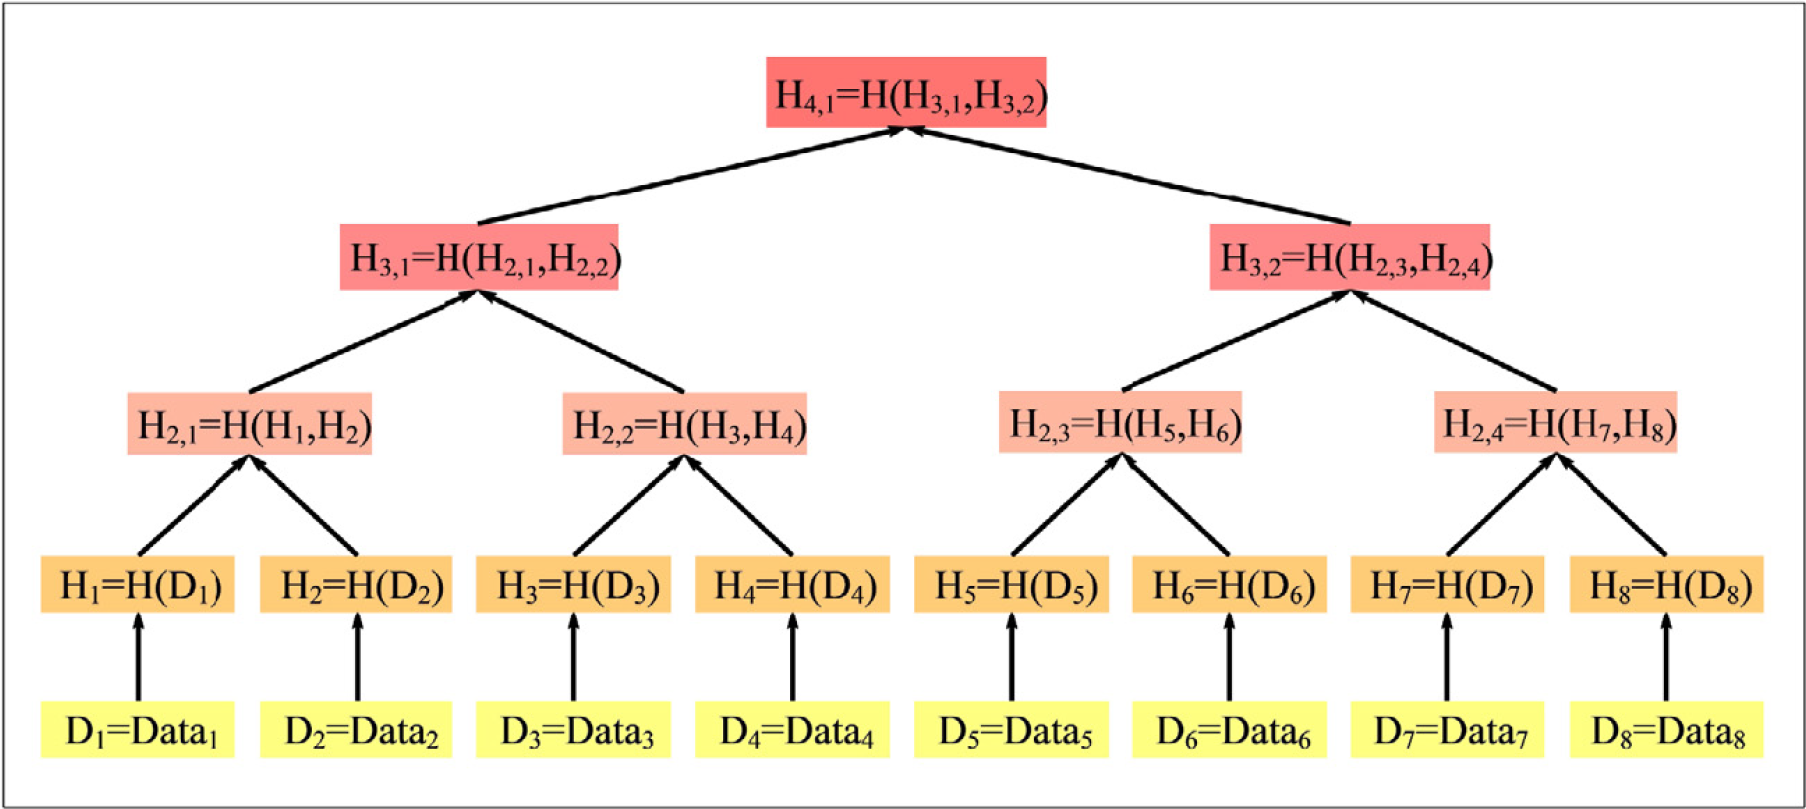
\includegraphics[width=1\linewidth]{merkle_tree.png}
    \caption{A Merkle tree created on 8 data points and  with hash function $H(\cdot)$, cited from \cite{zhu2021improved}}
    \label{fig:merkle_base}
\end{figure}

In 2021 an improvement was proposed for Merkle trees encoding electronic medical records (EMR) \cite{zhu2021improved}. The authors propose an algorithm that turns the usual Merkle structure (pictured Fig. \ref{fig:merkle_base}) into a convolution structure using some Kernel (pictured Fig. \ref{fig:cnn_merkle}), inspired by convolutional neural networks. 

\begin{figure}[H]
    \centering
    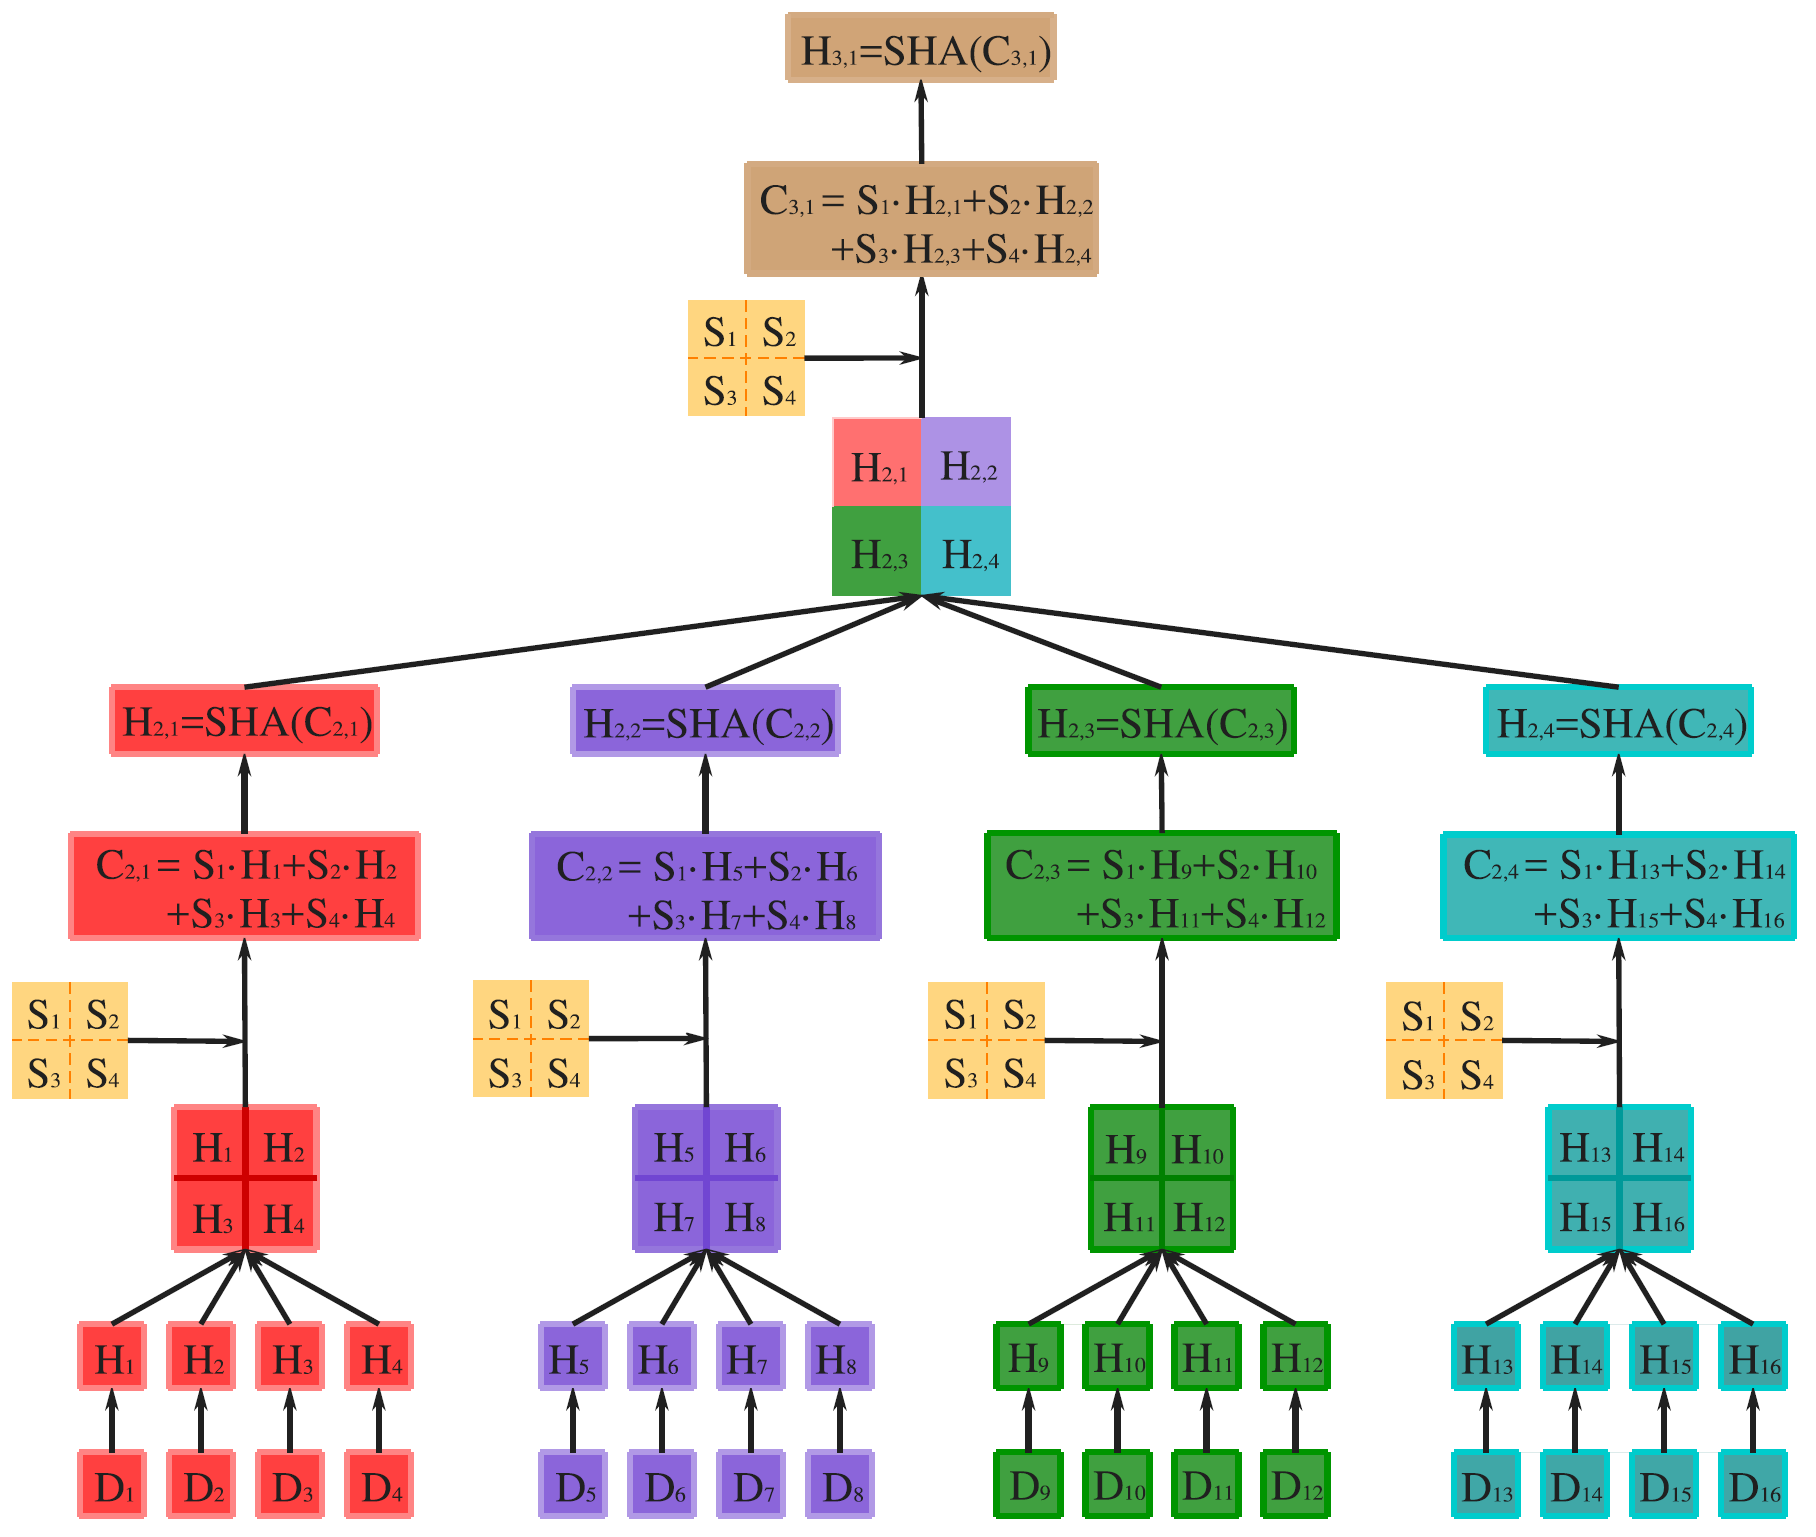
\includegraphics[width=1 \linewidth]{cnn_merkle.png}
    \caption{Layered Merkle tree with 16 data points, SHA256 hash function and $S$ convolution kernel, cited from \cite{zhu2021improved}}
    \label{fig:cnn_merkle}
\end{figure}

\noindent The example pictured requires the data to be able to be divided into 16 equal parts. This, however, is not a fixed number, it is dependent on the size of the kernel. Furthermore, noise can be added to 'fill out' the missing spots in the case of not enough data (e.g. 15 data blocks, one noise block in this case). This further increases privacy protection. Additionally, a significant speedup is proposed, as can be seen in Table \ref{tab:merkle_cnn_speed_diff}. Important to note, that this paper only considered this application in the EMR record and query application, it may not be guaranteed in different applications.



%\definecolor{SilverChalice}{rgb}{0.67,0.67,0.67}
\begin{table}
\centering
\caption{The difference between traditionaly k-ary merkle tree and the improved structure}
\label{tab:merkle_cnn_speed_diff}
\begin{tblr}{
  row{1} = {Gray,font=\bfseries},
  hlines,
  vlines,
}
Structure & Layer & Nodes                      & Hash calculations        \\
Original  & k*n+1 & $k^{2n+1}-1$               & $k^{2n}-1$               \\
Improved  & $n+1$ & $\frac{k^{2n+1}-1}{k^2-1}$ & $\frac{k^{2n}-1}{k^2-1}$ 
\end{tblr}
\end{table}

A significant potential upgrade to Merkle tree based systems are Recursive argument Merkle trees (Reckle trees) \cite{papamanthou2024reckle}. Papamanthou and their research group identified a gap in the calculations of proofs in Merkle trees, namely that they have to be fully recalculated, no matter the size of change in the data. Updatable batch proofs help blockchain systems efficiently compute and maintain proofs in a moving stream datablock setting. They propose and apply a technique called canonical hashing, allowing for batch proof updating in logarithmic time (though this requires sufficient parallelism, but provided that the speed would be batch size independent.) Canonical hashing is a recursive way to calculate a digest of a subset of leaves on the Merkle tree. This solution offers small memory footprint (112 KiB, independent of batch size), 10 to 15 times speed up on update time and 4.78 to 1485 times of speed up in verification under the right circumstances. While these results are likely to be well suited for industrial applications, they require too large resources for the proof of concept that is the scope of this thesis.\\
The paper by Liu et al. argues that the most popular form of hashing is Poseidon Hash for Merkle trees in the area of Zero-Knowledge Proofs (ZKP) \cite{liu2025acclmt}. Their identified research gap is how hardware acceleration can significantly speed up building Merkle trees with this type of hashing. While Poseidon is by default more expensive than traditional hashing (like SHA256) it scales better for certain hardware architecture and this is what this solution capitalizes on. Their proposed solution, AccIMT,  is a hardware-software combination that promises up to 1665 times speed up compared to other, software only solutions. Furthermore, it achieves 14.3 times speed and 14.8\% reduced area usage compared to previous state of art in similar tech. The proposed experiment setup optimized for blockchains and is at the time of writing unavailable for the purposes of thesis experimenting. This means while this solution is promising, it is both out of budget and out of scope for the thesis, while most likely promising a lucrative direction for further research.\\

The concept of Wibson-tree \cite{futoransky2020wibsontree} introduces a data market model consisting of 3 types of actors:
\begin{itemize}
    \item The Buyer: Looking for data from individuals, that belong to a criteria (e.g. age: 25-30, sex: female). Only receives whether a Seller is matching this criteria, nothing else. Unaware if the same Seller is participating in multiple data transactions.
    \item The Seller: An individual, choosing to sell their own data, anonymously. The Seller has no information about other Sellers participating in a transaction. Under certain circumstances, also unaware of the Buyer's criteria.
    \item The Notary: They are the supervising actor of the marketplace. They are able to validate the precision and quality of the Sellers data. They should not be able to learn anything else about the Seller. They get compensated for their work. They need to have public identities and off-chain reputation. \cite{travizano2020wibson}
\end{itemize}
The Buyer specifies a criterion $X_0$. The Notary assigns a 'Match Criterion' function to each Seller $\mathcal{S}$, such that:
\begin{equation*}
    F_{\mathcal{S}}(X) \in \{true, false\};\\
    \forall X \neq X_0:
\end{equation*}
The Buyer does not learn the value of $F_{\mathcal{S}}(X)$. If a Seller matches criterion $X_0$, they reveal, that $F_{\mathcal{S}}(X_0) = true$, and the valuation is the same as the one signed by the Notary (Sign$_{Notary} (F_\mathcal{S}) = true$).

Additionally the Notaries have to name a 'verification price', that they charge for their work unrelated to the actual outcome of the transaction (it successfully happens or not). This prevents the Buyers from creating unlimited queries for free.
Using this function, the Wibson-tree protocol builds a binary Merkle-tree-like structure with hashing, which allows for DAG and cryptographic proof creation. Proof is important, so the seller can be sufficiently identified on the blockchain and compensated after the data transaction successfully went through with the buyer.
Important to point out, while the design talks about, how the seller can withdraw consent to the data is sale, neither of the sources (\cite{futoransky2020wibsontree}, \cite{travizano2020wibson}) properly discuss exactly what happens and how in this given case.

\begin{figure}[H]
    \centering
    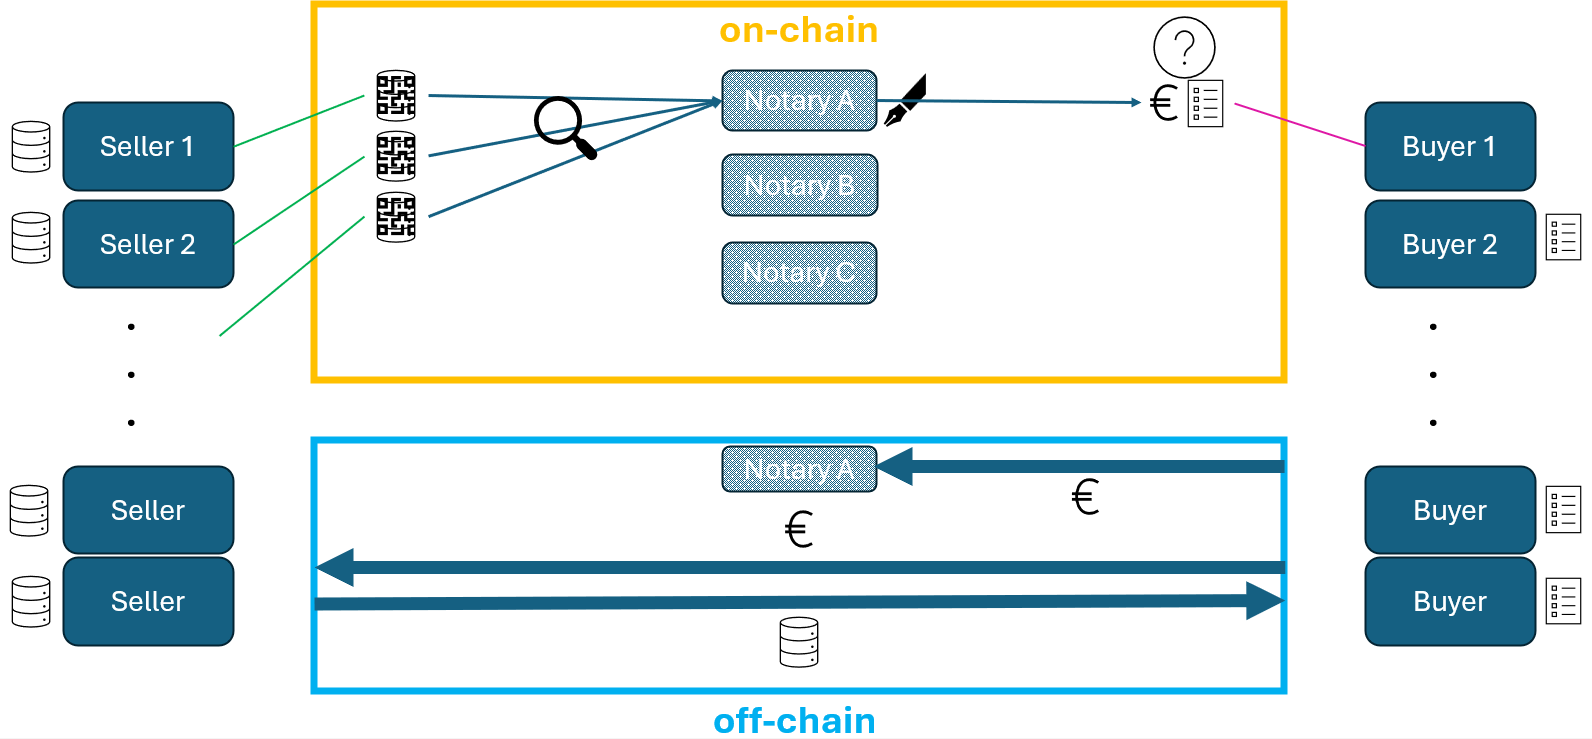
\includegraphics[width=1\linewidth]{wibson_tree.png}
    \caption{Wibson-protocol visualized}
    \label{fig:wib_tree_explain}
\end{figure}



This approach, however builds on raw data, that must be stored for the matching criterion to be calculated for every data request. In this form this can lead to PII leaks.
This warrants the need for a 2-step process, that anonymises the data first, then calculates the criterion.
The first step can be a good aggregation process, that generates a non-retraceable output. Then this can be 'fed' into the matching criterion and provide data to buyers this way.
Another good option is to collect already in a way that gives it some secrecy (e.g. age range, instead of age, geographical polygon instead of city). This, however is not possible with all kinds of information, those will need a case-by-case analysis.
Using the Wibson protocol, the seller can only get verification for the anonymised data. It's important to invent a way to be able for the proof to be connected back to the original Seller.

\chapter{Methodology and design}
\section{Research problems}
Based on the results and the gaps of the literature review and the business request of the company (Namely to build a scalable data marketplace model, that is human-centric and ethical by design) the following research question are posed:\\
\textbf{RQ 1}: Can a system designed for commercial use operate on at least the FACT principles? (Preferably conform to other ethical guidelines too)?\\
\textbf{RQ 2}:Is a 2-step data collection and criterion matching process sufficient to create a wibson-like protocol for ethical data economy model?\\
\textbf{RQ 3}:What proof can be generated, that still allow for the seller to be rewarded? % to be revised

\section{WIP: possible business scenarios}\label{sec: business_scen}
Designing this framework requires it to function in certain ways, given certain scenarios. Here we discuss two of the most likely cases that this system would be used in. We indicate:
\begin{itemize}
    \item the stakeholders,
    \item the data collected and used,
    \item the sensitivity of different types of data,
    \item how this data is likely to be used and what the path of said data is,
    \item and finally analyze what critical functions the case requires and what are dangerous aspects, if any.
\end{itemize} 
The three scenarios analyzed here are a marketing campaign, a product development case and service provider self-improvement. The data involved in these cases is discussed in a manner that is realistic with regard of Fixmeapp business model as a booking company and what data could be realistically collected this way.

\subsection{Case 1: Marketing campaign}
In this first likely business case, the buyer would use the bought data for launching a marketing campaign. This can mean a marketing company or a marketing department of e.g. a skincare product company. The stakeholders in this case are; the buyer (Marketing team/company), Governor (Fixmeapp), User(s). The data collected and stored about the user through bookings are manifold and most of it is quite valuable for the buyer in this case. The data in question in no particular order:
\begin{itemize}
    \item Geographical polygon data (same idea as can be seen with Wibson protocol \cite{futoransky2020wibsontree})
    \item Demographic data (age, biological sex OR gender, etc.)
    \item Booking history (with one particular company or all together, frequency can be inferred from these)
    \item (Based on booking history and geographical polygon, some sort of salary range can be inferred) % maybe? source?
\end{itemize}
Geographical polygon data and demographic data (for example; a male in their 30's, living in the general East-Uusimaa area) is not PII. Note, if the geographical polygon is not defined carefully/generally enough, it can lead to some sort of identification, combined with other data. Booking history with a particular partner in general is not sensitive, if stored correctly. (Bad example: male hair dying from blond to brunette, 10:30, [date], [saloon location]; Good example: male hair dying, [morning/afternoon/after work hours]). Data presented and purchased this way can be used to narrow down customer personas/profiles. These then can be used to design adverts or discount campaigns that accurately hit these customers, be it for retention or expanding client circles.\\
In this example the data would be generated by the users through booking, sent and stored by Fixmeapp and be bought by the marketing departments/companies, that the users would be informed about. This process does not protect users against data reselling by the marketing companies, that could be for example a contractual obligation for the parties involved.\\

\subsection{Case 2: Product development}
In this business case the buyer acquires data in order to develop an existing or new product, based on users of e.g. 
beautician services and the providers themselves. The stakeholders in this case are; the buyer (Product company), Governor (Fixmeapp), User(s) and Provider(s). The relevant data is much more narrow in this case, than the previous one, as much of the useful information, like what climate the product will be used in, has to be inferred from e.g. geographical polygons. Information that can prove useful:
\begin{itemize}
    \item Geographical polygon data. For inferring weather and humidity conditions, (tap) water quality.
    \item Demographic data (age, biological sex OR gender, etc.). This allows the producer to paint an accurate customer persona
    \item Booking history. For the same reasons as above. (Which saloons buy it, what kind of people want to use them)
    \item Allergies. There may be skin allergies affecting a larger portion of the customer population, that has to be taken into account when developing the recipe.
\end{itemize}
The first two bullet points still do not qualify as PII, given they are collected and stored in a reasonable manner. Booking history of a particular kind of provider (beautician - skin care, hairdresser - hair products, etc.) is in vast majority of the cases not enough to enable identification of any individual. Allergies, are however, different. This is health record data and should be stored and handled accordingly. \\
Similarly as the previous example, the data would be generated by the users through booking, sent and stored by Fixmeapp and be bought by companies, that the users would be informed about. This process does not protect users against data reselling by the marketing companies, that could be for example a contractual obligation for the parties involved. This second part is crucial in this case, as we are dealing with data qualifying as health record.\\

\subsection{Case 3: Service provider}
In this business case the service providers (at whom the users can book services through Fixmeapp's platform) want to improve the services they offer. They need data generated by the booking customers to see the pain points/shortcomings of their services (e.g. wrong opening hours, not offering a popular service).
The stakeholders in this case are; the buyer (Provider), Governor (Fixmeapp), User(s). The relevant data are things that are directly connected to the booking, circumstances of these and aftercare (e.g. ratings, what the user liked, what they did not like). More accurately:
\begin{itemize}
    \item Geographical polygon data. To understand the general range where they attract customers from and where they have competition because of this.
    \item Demographic data (age, biological sex OR gender, etc.). The sort of people booking their and similar services.
    \item Booking history. How often customers return, how often they go to competition for similar services, potentially what sort of other services they book together with the services provided by the provider.
    \item Ratings and complaint data. Crucial for identifying customer needs and pain points.
    \item (Based on booking history and geographical polygon, some sort of salary range can be inferred. This can help with pricing strategies.)
\end{itemize}
Just as with the other two examples, the first two points should not be able to be used for identification of a person. Combined with booking information, these all together should still not be enough to identify a person. Information acquired this way about competition should also not conflict with existing legal frameworks. (Prices, services available, products used are types of information, that a throughout competition analysis could reveal.) All listed data is can be used to define competitive pricing and cater to a more optimized audience. The path of the data should be traceable throughout its journey, however an identical problem to the previous two cases arises; there is no way to guarantee protection against reselling the data.
All the business cases feature problems with secondary data markets or data reselling. This will be addressed later in this chapter, under Section \ref{sec:attack_surf}.

\section{Design decisions}
A data contribution system like this naturally poses a series of design questions. Firstly, while the solution is mostly based on the Wibson-tree concept, there are several significant differences to it, when compared. The most important topic is probably centralisation. Originally the Wibson-system was designed to serve a marketplace of several Sellers, less, but still significant amount of Buyers and Notaries. These Notaries can be either individuals or legal entities, who possess ground truth on the sellers' information and are able to verify it, while having public identities and a verifiable off-chain reputation. \cite{travizano2020wibson}
They are not assigned to transactions automatically, if an entity qualifies, their role as a Notary is an agreement of all parties.
As anyone can take on any role, so long as they qualify and there exists no central authority/control figure makes the concept decentralized in core.\\
Fixmeapp's use case differs in this aspect; For user data transactions they position themselves as the Notary and to some degree the Seller. Table \ref{tab:decentral_compare} shows what trade-offs this means:\\

\begin{table}[h!]
\centering
\caption{Comparison of the decentralized and centralized approaches.}
\label{tab:decentral_compare}
\begin{tabular}{llllllllll}
\cellcolor[HTML]{343434}{\color[HTML]{FFFFFF} Aspects} & \cellcolor[HTML]{343434}{\color[HTML]{FFFFFF} Decentralized marketplace} & \cellcolor[HTML]{343434}{\color[HTML]{FFFFFF} \begin{tabular}[c]{@{}l@{}}Non-conventional\\ centralized marketplace\\ (Fixmeapp)\end{tabular}} &  &  &  &  &  &  &  \\ \cline{1-3}
\multicolumn{1}{|l|}{\cellcolor[HTML]{C0C0C0}Authority figure} & \multicolumn{1}{l|}{\cellcolor[HTML]{C0C0C0}None} & \multicolumn{1}{l|}{\cellcolor[HTML]{C0C0C0}Governor (Fixmeapp)} &  &  &  &  &  &  &  \\ \cline{1-3}
\multicolumn{1}{|l|}{\cellcolor[HTML]{C0C0C0}Query interaction participants} & \multicolumn{1}{l|}{\cellcolor[HTML]{C0C0C0}Seller, Buyer, Notary} & \multicolumn{1}{l|}{\cellcolor[HTML]{C0C0C0}User, Service provider, Governor} &  &  &  &  &  &  &  \\ \cline{1-3}
\multicolumn{1}{|l|}{\cellcolor[HTML]{C0C0C0}Data storage} & \multicolumn{1}{l|}{\cellcolor[HTML]{C0C0C0}\begin{tabular}[c]{@{}l@{}}Client side, reference of the \\ data is on the blockchain.\end{tabular}} & \multicolumn{1}{l|}{\cellcolor[HTML]{C0C0C0}\begin{tabular}[c]{@{}l@{}}SQL database, reference to\\  the data in The Marketplace\end{tabular}} &  &  &  &  &  &  &  \\ \cline{1-3}
\multicolumn{1}{|l|}{\cellcolor[HTML]{C0C0C0}Data auditor} & \multicolumn{1}{l|}{\cellcolor[HTML]{C0C0C0}Notary} & \multicolumn{1}{l|}{\cellcolor[HTML]{C0C0C0}Governor (Fixmeapp)} &  &  &  &  &  &  &  \\ \cline{1-3}
\multicolumn{1}{|l|}{\cellcolor[HTML]{C0C0C0}\begin{tabular}[c]{@{}l@{}}Compensation currency\\  for the Sellers and Notaries\end{tabular}} & \multicolumn{1}{l|}{\cellcolor[HTML]{C0C0C0}Cryptocurrency tokens} & \multicolumn{1}{l|}{\cellcolor[HTML]{C0C0C0}\begin{tabular}[c]{@{}l@{}}Fixmeapp internal \\ economy tokens\end{tabular}} &  &  &  &  &  &  &  \\ \cline{1-3}
\multicolumn{1}{|l|}{\cellcolor[HTML]{C0C0C0}Wallet type} & \multicolumn{1}{l|}{\cellcolor[HTML]{C0C0C0}Ethereum Master Wallet} & \multicolumn{1}{l|}{\cellcolor[HTML]{C0C0C0}User account wallet} &  &  &  &  &  &  &  \\ \cline{1-3}
\multicolumn{1}{|l|}{\cellcolor[HTML]{C0C0C0}Entities receiving compensation} & \multicolumn{1}{l|}{\cellcolor[HTML]{C0C0C0}Seller, Notary} & \multicolumn{1}{l|}{\cellcolor[HTML]{C0C0C0}User, Governor} &  &  &  &  &  &  &  \\ \cline{1-3}
\end{tabular}
\end{table}

\noindent{For} the company this is of course the more beneficial case, while still keeping to the original protocol in privacy aspects. For the rest of thesis, the definitions will change as following:
\begin{itemize}
    \item \textbf{User(s)}: The producers and owner's of the 'user data'. Any transactions involving the User's data will earn compensation for the User. They are not selling the data themselves, but they do consent to their data being part of the economy and which parts may be.
    \item \textbf{Service provider(s)}: They are the buyers of the Users' data. They require the data to provide the services to the users booked through the Fixmeapp platform. Further more they can make queries to the Governor for market or advertising research to buy user data.
    \item \textbf{Governor (Fixmeapp)}: They take on the Notary duties (verifying matches and signing them), as well as responding to queries by Service providers. This way they are the one that actually sells the data and takes a cut from the income generated by the transaction and forwards the rest to the Users.
\end{itemize}
The next design objective is regarding data encryption. It is important to decide when and where raw(unencrypted) data is stored/used, as well as when and how many times an encryption action is performed on the data. This study considers three probable designs for this.\\
First and most intuitively we consider the Wibson-protocol. It operates on a decentralized model, with heavy user interaction; The Users have their data stored client side, with a hashed reference (created by Merkle-tree encoding) on a blockchain, that is then queried by the Service providers, but each user has to individually respond to this query. This would require near-constant user activity on a marketplace for most of the userbase for the data to be considered statistically significant. In the case of booking apps, such as Fixmeapp, this near-constant activity of most of the userbase is not realistic to achieve, as booking applications are used on average three times a week %placeholder number
[citation required].\\
Second consideration was applying the Wibson-protocol, but the Governor entity stores all the raw user data. The Users have a choice in what is being stored and what of that can be shared. For the data transactions the Governor makes statistics/aggregation of user data available to the Buyers (advertises) about the userbase when queried. These queries still take resource investment from the Buyers, so they can not infinitely query. If the Buyers deem the data valuable enough to purchase, the Governor confirms the validity and accuracy of the stored data, and if it is up to standards, completes the transaction and sends users their compensation. This version does not require a near-constant userbase activity, while still holding up standards of ethicality, as Users decide what data can be shared about them and this consent is withdrawable at any time. This, however heavily relies on a secure data storage method, as storing data unencrypted is a major threat in case of a data leak. Encryption happens on every query, similarly to the previous case.\\
Third consideration was an encrypted storage [LOOK AT EDITOR] %Carlos, can we just have the Governor store hashes and have the raw stuff client side? is that like something? We still need some database statistics, but I see this is as a possible out?

After careful consideration of all three design paths, the third one wins out on...


\section{Handling User Data}
After discussing, how is it most optimal to deal with and store data, now we need to consider what type of data the project is handling. This section will be divided into two topics: What sort of data is queried and based on that what sort of data should we collect from the users, to fulfill these needs best to our ability.\\
As can be seen from the business cases the data we need to collect is 
\begin{itemize}
    \item Geographical polygon,
    \item Demographic data,
    \item Contact data (this is purely for the booking functionality),
    \item Booking history,
    \item Ratings and complaint data,
    \item Allergies to relevant products.
\end{itemize}
% everything below here is WIP and will be completed with the proof of concept
The first two items should be collected in a bucketed way, as in creating a mapping between values and the buckets (age - age range, city - polygon). Contact information is something that is only a technical requirement, so it needs to be encrypted and preferably stored separately from other data, that will be used in the data market. Booking history, as discussed in Section \ref{sec: business_scen}, needs to be stored in a way, that makes identification of an individual difficult. It also needs to be stored in a way, that supports regular updates. Ratings and complaint data should be similar, however it is more sensible to store it connected to the service providers, rather than the individuals. Allergies are considered health data, thus should be handled according to the relevant regulations per region.


\section{Attack surfaces}\label{sec:attack_surf}
%WIP
One of the main problems the system faces is already laid out by \cite{hyrynsalmi2023balancing}. Soon as data leaves our system, transparency, user protection and reselling protection can no longer be guaranteed by the system. Data (and other digital goods) need to be decrypted or "released from protection" to be consumed, to be used. This is known as the 'analog hole' in Digital Rights Management \cite{haber2003if}. Even tough the terms is 'overly restrictive' in the words of the author, as even this case is still in a digital form, the takeaway is that using purely software solutions it is not plausible to protect the product, in this case data. To address this there should be policies held up by trust and/or law (most likely in the form of inter-organizational contracts). Even this gives little protection against truly malevolent actors, even if we were to consider blockchain as a solution. This attack surface proves that (ethical) data governance needs both technical and legal layers for defense.



\begin{figure}[h] % In general this is the code for figures
\centering %centering if needed

\includegraphics[scale=0.5]{elte-logo.jpg} %scaling if needed, picture has to be in the same folder as the .tex file
\caption{If you need notes for the figure, use this}
\end{figure}


\chapter{Proof of concept}
\section{Subchapter}
...

\chapter{Discussion and conclusions}
...
%\section{Theroem style}
%\begin{theorem} [Namer of the Theorem] \label{theorem1}
%This is a theorem
%\end{theorem}

%\begin{proof}
%And this is the proof, which contains an equation:
%\begin{equation} \label{eq1}
%1+1=2
%\end{equation}
%End of proof.
%\end{proof}

%\begin{defi}
%This is a definiton, the numbering goes together with theorems.
%\end{defi}

%\begin{claim}
%You can reference an equation the following way: \eqref{eq1}, theorem: \ref{theorem1}.
%\end{claim}

%\begin{note}
%This is a note
%\end{note}

%\begin{conseq}
%This is a consequence
%\end{conseq}

%\begin{eg}
%This is an example
%\end{eg}

\section{Source code}
\begin{verbatim}
   this is the source code
\end{verbatim}

\newpage

\bibliography{bibexample} % just insert the bib file name, without .bib, it has to be in the same folder as the .tex file, 
%%%%%%%%%%%%%% separate the bib files with a comma inside the parenthesis
\bibliographystyle{alpha}



\end{document}
